%===============================================================================
% LaTeX sjabloon voor de bachelorproef toegepaste informatica aan HOGENT
% Meer info op https://github.com/HoGentTIN/latex-hogent-report
%===============================================================================

\documentclass[dutch,dit,thesis]{hogentreport}

% TODO:
% - If necessary, replace the option `dit`' with your own department!
%   Valid entries are dbo, dbt, dgz, dit, dlo, dog, dsa, soa
% - If you write your thesis in English (remark: only possible after getting
%   explicit approval!), remove the option "dutch," or replace with "english".

\usepackage{lipsum} % For blind text, can be removed after adding actual content

%% Pictures to include in the text can be put in the graphics/ folder
\graphicspath{{graphics/}}

%% For source code highlighting, requires pygments to be installed
%% Compile with the -shell-escape flag!
\usepackage[section]{minted}
%% If you compile with the make_thesis.{bat,sh} script, use the following
%% import instead:
%% \usepackage[section,outputdir=../output]{minted}
\usemintedstyle{solarized-light}
\definecolor{bg}{RGB}{253,246,227} %% Set the background color of the codeframe

%% Change this line to edit the line numbering style:
\renewcommand{\theFancyVerbLine}{\ttfamily\scriptsize\arabic{FancyVerbLine}}

%% Macro definition to load external java source files with \javacode{filename}:
\newmintedfile[javacode]{java}{
    bgcolor=bg,
    fontfamily=tt,
    linenos=true,
    numberblanklines=true,
    numbersep=5pt,
    gobble=0,
    framesep=2mm,
    funcnamehighlighting=true,
    tabsize=4,
    obeytabs=false,
    breaklines=true,
    mathescape=false
    samepage=false,
    showspaces=false,
    showtabs =false,
    texcl=false,
}

% Other packages not already included can be imported here

%%---------- Document metadata -------------------------------------------------
% TODO: Replace this with your own information
\author{Bram Lippens}
\supervisor{Dhr. B. Vertonghen}
\cosupervisor{Dhr. S. Hilleart}
\title[Optionele ondertitel]%
    {Welke 2D game engines zijn geschikt voor programmeurs van AllPhi met een C\# achtergrond maar geen game development achtergrond om games te ontwikkelen voor evenementen?}
\academicyear{\advance\year by -1 \the\year--\advance\year by 1 \the\year}
\examperiod{1}
\degreesought{\IfLanguageName{dutch}{Professionele bachelor in de toegepaste informatica}{Bachelor of applied computer science}}
\partialthesis{false} %% To display 'in partial fulfilment'
%\institution{Internshipcompany BVBA.}

%% Add global exceptions to the hyphenation here
\hyphenation{back-slash}

%% The bibliography (style and settings are  found in hogentthesis.cls)
\addbibresource{bachproef.bib}            %% Bibliography file
\addbibresource{../voorstel/voorstel.bib} %% Bibliography research proposal
\defbibheading{bibempty}{}

%% Prevent empty pages for right-handed chapter starts in twoside mode
\renewcommand{\cleardoublepage}{\clearpage}

\renewcommand{\arraystretch}{1.2}

%% Content starts here.
\begin{document}

%---------- Front matter -------------------------------------------------------

\frontmatter

\hypersetup{pageanchor=false} %% Disable page numbering references
%% Render a Dutch outer title page if the main language is English
\IfLanguageName{english}{%
    %% If necessary, information can be changed here
    \degreesought{Professionele Bachelor toegepaste informatica}%
    \begin{otherlanguage}{dutch}%
       \maketitle%
    \end{otherlanguage}%
}{}

%% Generates title page content
\maketitle
\hypersetup{pageanchor=true}

%%=============================================================================
%% Voorwoord
%%=============================================================================

\chapter*{\IfLanguageName{dutch}{Woord vooraf}{Preface}}%
\label{ch:voorwoord}

%% TODO:
%% Het voorwoord is het enige deel van de bachelorproef waar je vanuit je
%% eigen standpunt (``ik-vorm'') mag schrijven. Je kan hier bv. motiveren
%% waarom jij het onderwerp wil bespreken.
%% Vergeet ook niet te bedanken wie je geholpen/gesteund/... heeft

\lipsum[1-2]
%%=============================================================================
%% Samenvatting
%%=============================================================================

% TODO: De "abstract" of samenvatting is een kernachtige (~ 1 blz. voor een
% thesis) synthese van het document.
%
% Een goede abstract biedt een kernachtig antwoord op volgende vragen:
%
% 1. Waarover gaat de bachelorproef?
% 2. Waarom heb je er over geschreven?
% 3. Hoe heb je het onderzoek uitgevoerd?
% 4. Wat waren de resultaten? Wat blijkt uit je onderzoek?
% 5. Wat betekenen je resultaten? Wat is de relevantie voor het werkveld?
%
% Daarom bestaat een abstract uit volgende componenten:
%
% - inleiding + kaderen thema
% - probleemstelling
% - (centrale) onderzoeksvraag
% - onderzoeksdoelstelling
% - methodologie
% - resultaten (beperk tot de belangrijkste, relevant voor de onderzoeksvraag)
% - conclusies, aanbevelingen, beperkingen
%
% LET OP! Een samenvatting is GEEN voorwoord!

%%---------- Nederlandse samenvatting -----------------------------------------
%
% TODO: Als je je bachelorproef in het Engels schrijft, moet je eerst een
% Nederlandse samenvatting invoegen. Haal daarvoor onderstaande code uit
% commentaar.
% Wie zijn bachelorproef in het Nederlands schrijft, kan dit negeren, de inhoud
% wordt niet in het document ingevoegd.



%%---------- Samenvatting -----------------------------------------------------
% De samenvatting in de hoofdtaal van het document

\chapter*{\IfLanguageName{dutch}{Samenvatting}{Abstract}}

TODO


%---------- Inhoud, lijst figuren, ... -----------------------------------------

\tableofcontents

% In a list of figures, the complete caption will be included. To prevent this,
% ALWAYS add a short description in the caption!
%
%  \caption[short description]{elaborate description}
%
% If you do, only the short description will be used in the list of figures

\listoffigures

% If you included tables and/or source code listings, uncomment the appropriate
% lines.
%\listoftables
%\listoflistings

% Als je een lijst van afkortingen of termen wil toevoegen, dan hoort die
% hier thuis. Gebruik bijvoorbeeld de ``glossaries'' package.
% https://www.overleaf.com/learn/latex/Glossaries

%---------- Kern ---------------------------------------------------------------

\mainmatter{}

% De eerste hoofdstukken van een bachelorproef zijn meestal een inleiding op
% het onderwerp, literatuurstudie en verantwoording methodologie.
% Aarzel niet om een meer beschrijvende titel aan deze hoofdstukken te geven of
% om bijvoorbeeld de inleiding en/of stand van zaken over meerdere hoofdstukken
% te verspreiden!

%%=============================================================================
%% Inleiding
%%=============================================================================

\chapter{\IfLanguageName{dutch}{Inleiding}{Introduction}}%
\label{ch:inleiding}

De inleiding moet de lezer net genoeg informatie verschaffen om het onderwerp te begrijpen en in te zien waarom de onderzoeksvraag de moeite waard is om te onderzoeken. In de inleiding ga je literatuurverwijzingen beperken, zodat de tekst vlot leesbaar blijft. Je kan de inleiding verder onderverdelen in secties als dit de tekst verduidelijkt. Zaken die aan bod kunnen komen in de inleiding~\autocite{Pollefliet2011}:

\begin{itemize}
  \item context, achtergrond
  \item afbakenen van het onderwerp
  \item verantwoording van het onderwerp, methodologie
  \item probleemstelling
  \item onderzoeksdoelstelling
  \item onderzoeksvraag
  \item \ldots
\end{itemize}

\section{\IfLanguageName{dutch}{Probleemstelling}{Problem Statement}}%
\label{sec:probleemstelling}

AllPhi is een technologiebedrijf dat jaarlijks deelneemt aan verschillende technologiebeurzen, waar het een interactieve uitdaging voor bezoekers organiseert. Voor de meest recente editie van de uitdaging ontwikkelde AllPhi een eigen Snake-spel, gebouwd met behulp van C\# en .NET. Ondanks dat de medewerkers van AllPhi geen professionele gameontwikkelaars zijn, waren ze tevreden met het resultaat.

Het onderzoek zal resulteren in een beknopte lijst van geselecteerde game-engines die als potentieel geschikt worden beschouwd voor het ontwikkelen van een `Space Invaders`-achtig spel. Uit deze lijst zal een game-engine worden gekozen voor de ontwikkeling van een proof-of-concept. Dit proof-of-concept zal fungeren als praktisch demonstratiemiddel, waardoor AllPhi in staat zal zijn om nieuwe spellen te creëren voor gebruik op verschillende evenementen.


\section{\IfLanguageName{dutch}{Onderzoeksvraag}{Research question}}%
\label{sec:onderzoeksvraag}

Met als doel het verbeteren van toekomstige uitdagingen, wil AllPhi onderzoeken welke game-engine het meest toegankelijk is voor mensen met een achtergrond in C\# en .NET, maar zonder ervaring in game-ontwikkeling.

\section{\IfLanguageName{dutch}{Onderzoeksdoelstelling}{Research objective}}%
\label{sec:onderzoeksdoelstelling}

De kern van deze paper is het verstrekken van aanbevelingen aan AllPhi met betrekking tot geschikte game-engines voor de ontwikkeling van een `Space Invaders`-achtig spel. Dit wordt bereikt door middel van een grondig onderzoek dat een uitgebreide analyse omvat van beschikbare game-engines die geschikt zijn voor dit specifieke genre.

\section{\IfLanguageName{dutch}{Opzet van deze bachelorproef}{Structure of this bachelor thesis}}%
\label{sec:opzet-bachelorproef}

% Het is gebruikelijk aan het einde van de inleiding een overzicht te
% geven van de opbouw van de rest van de tekst. Deze sectie bevat al een aanzet
% die je kan aanvullen/aanpassen in functie van je eigen tekst.

De rest van deze bachelorproef is als volgt opgebouwd:

In Hoofdstuk~\ref{ch:stand-van-zaken} wordt een overzicht gegeven van de stand van zaken binnen het onderzoeksdomein, op basis van een literatuurstudie.

In Hoofdstuk~\ref{ch:methodologie} wordt de methodologie toegelicht en worden de gebruikte onderzoekstechnieken besproken om een antwoord te kunnen formuleren op de onderzoeksvragen.

% TODO: Vul hier aan voor je eigen hoofstukken, één of twee zinnen per hoofdstuk
In Hoofdstuk~\ref{ch:proof-of-concept} wordt er een proof of concept uitgewerkt in een van de engines die geschikt zijn voor AllPhi.

In Hoofdstuk~\ref{ch:conclusie}, tenslotte, wordt de conclusie gegeven en een antwoord geformuleerd op de onderzoeksvragen. Daarbij wordt ook een aanzet gegeven voor toekomstig onderzoek binnen dit domein.
\chapter{\IfLanguageName{dutch}{Stand van zaken}{State of the art}}%
\label{ch:stand-van-zaken}

% Tip: Begin elk hoofdstuk met een paragraaf inleiding die beschrijft hoe
% dit hoofdstuk past binnen het geheel van de bachelorproef. Geef in het
% bijzonder aan wat de link is met het vorige en volgende hoofdstuk.

% Pas na deze inleidende paragraaf komt de eerste sectiehoofding.
\section{Low Code}


\section{\IfLanguageName{dutch}{Game Engines}{Game Engines}}%
\label{sec:game-engines}
De term "game engine" kwam op in het midden van de jaren 1990, met de opkomst van het razend populaire videospel Doom, ontwikkeld door id Software. Doom was een van de spellen die een revolutie teweegbrachten in de videogame-industrie. Het spel was opgebouwd uit twee lagen: de kernsoftwarecomponenten, zoals het renderingsysteem voor de driedimensionale omgeving, de collisiedetectie en het geluidssysteem, en de andere laag, die het ontwerp van het spel, de werelden/niveaus en de spelregels omvatte. Hierdoor kon id Software nieuwe iteraties van videospellen uitbrengen met verschillende looks, nieuwe unieke werelden en nieuwe spelregels, zonder ingrijpende aanpassingen aan de kerncomponenten te hoeven maken. Dit leidde tot de term "game engine". \cite{gregory2018game}

\subsection{GameMaker studio 2}
GameMaker Studio 2, een engine die geschikt is voor beginners om 2D-games te maken, maakt gebruik van een drag-and-drop interface en vereist geen extra programmeertaal naast C\#. Het gebruikt zijn eigen taal genaamd GameMaker Language (GML). \autocite{cossu2019game}

\subsection{Unity}
Een ander opmerkelijk voorbeeld is Unity, een commerciële game engine die een breed scala aan functionaliteiten biedt. Naast ondersteuning voor zowel 2D- als 3D-graphics, biedt Unity ook geavanceerde mogelijkheden op het gebied van fysica, geluid, netwerken en augmented reality. Dit maakt Unity een populaire keuze onder ontwikkelaars voor het creëren van diverse en innovatieve game-ervaringen. \autocite{Haas2014}

\subsection{Godot}
Godot, een gratis en open-source platform, biedt een uitstekende combinatie van toegankelijkheid en flexibiliteit, zonder verborgen functionaliteiten achter een betaalmuur. Wat Godot verder onderscheidt, is de levendige en ondersteunende gemeenschap die het omringt. Deze gemeenschap draagt bij aan het continue verbeteren en uitbreiden van de mogelijkheden van het platform, waardoor ontwikkelaars profiteren van een schat aan kennis, ondersteuning en gedeelde middelen. \autocite{Bradfield2018}

In Godot vormen nodes de bouwstenen voor het maken van spellen. Een node is een object dat gespecialiseerde spelfunctionaliteit vertegenwoordigt, zoals het weergeven van een scherm, afspelen van animaties of modellen. Elke node heeft verschillende eigenschappen waarmee het gedrag kan worden geconfigureerd. Het modulaire systeem maakt het toevoegen van nodes flexibel en efficiënt. \autocite{Bradfield2018}

Het scripten in Godot kan worden gedaan in drie verschillende talen. GDScript is de standaardtaal binnen Godot en staat het dichtst bij de engine zelf. C# kan ook worden gebruikt, maar wordt meestal ingezet voor optimalisatiedoeleinden. Godot ondersteunt echter een flexibele combinatie van deze twee talen.\autocite{Bradfield2018} VisualScript was een derde optie, maar deze taal wordt niet langer ondersteund sinds de release van Godot 4.0.

\subsection{Unreal Engine 4}
Unreal Engine 4 omvat een breed scala aan componenten die verschillende aspecten van game-ontwikkeling bestrijken, waaronder sound engines, physics engines, graphics engines, gameplay frameworks en online functionaliteiten. Een van de meest opvallende kenmerken is de Unreal Editor, een krachtige ontwikkelomgeving waarin spellen worden geprogrammeerd en ontworpen. De editor biedt een reeks modules, zoals Material en Blueprint, die ontwikkelaars in staat stellen om op een intuïtieve manier complexe game-elementen te maken en te beheren. Met deze uitgebreide set tools en functies stelt Unreal Engine 4 ontwikkelaars in staat om hoogwaardige, interactieve ervaringen te creëren binnen een geavanceerde en veelzijdige ontwikkelomgeving. \autocite{lee2016learning}

\subsubsection{Blueprints}
Het woord "Blueprint" heeft verschillende betekenissen binnen Unreal Engine 4. Aan de ene kant verwijst het naar een door Epic Games ontwikkelde scripttaal specifiek voor Unreal Engine 4. Aan de andere kant wordt het gebruikt om te verwijzen naar een nieuw type spelobject dat is gemaakt met behulp van Blueprint-functionaliteit.
\autocite{romero2019blueprints}

\subsection{Buildbox}
Buildbox is specifiek ontworpen voor het ontwikkelen van 2D-games en staat bekend om zijn vermogen om ontwikkelaars in staat te stellen snel spellen te creëren en te exporteren naar diverse platforms, waaronder mobiele telefoons. Met een intuïtieve interface en een krachtige set aan tools, stelt Buildbox gebruikers in staat om zonder uitgebreide programmeerkennis complexe 2D-games te ontwikkelen. Het platform biedt ook uitgebreide mogelijkheden voor het aanpassen van gameplay-elementen en het ontwerpen van visueel aantrekkelijke spelomgevingen, waardoor ontwikkelaars hun creativiteit volledig kunnen benutten. Met Buildbox kunnen ontwikkelaars snel en efficiënt hoogwaardige 2D-games produceren die geschikt zijn voor een breed scala aan apparaten en platforms. \autocite{audronis2016buildbox}

\subsection{Construct 3}
Construct 3 is een geavanceerde HTML5-gebaseerde 2D-game engine die bekend staat om zijn ondersteuning voor visueel programmeren. Met een intuïtieve interface en krachtige tools stelt Construct 3 gebruikers in staat om spellen te ontwikkelen zonder dat er diepgaande programmeerkennis vereist is. Een opvallend kenmerk van Construct 3 is zijn vermogen om spellen te exporteren naar een breed scala aan platforms, waaronder Windows, MacOS, Linux en mobiele telefoons. Deze flexibiliteit stelt ontwikkelaars in staat om hun creaties gemakkelijk beschikbaar te maken voor een groot publiek, ongeacht het apparaat dat ze gebruiken. Met Construct 3 kunnen ontwikkelaars snel en efficiënt hoogwaardige 2D-games maken en deze distribueren naar verschillende doelplatforms. \autocite{enwiki:1200994136}

\subsection{Phaser}

\subsection{Love2D}

\subsection{Stencyl}

\subsection{Torque 2D}

\subsection{GDevelop}

\subsection{Pixel Game Maker MV}

\subsection{Solar2D}

\subsection{Pico-8}

\subsection{GameSalad}
%%=============================================================================
%% Methodologie
%%=============================================================================

\chapter{\IfLanguageName{dutch}{Methodologie}{Methodology}}%
\label{ch:methodologie}

%% TODO: In dit hoofstuk geef je een korte toelichting over hoe je te werk bent
%% gegaan. Verdeel je onderzoek in grote fasen, en licht in elke fase toe wat
%% de doelstelling was, welke deliverables daar uit gekomen zijn, en welke
%% onderzoeksmethoden je daarbij toegepast hebt. Verantwoord waarom je
%% op deze manier te werk gegaan bent.
%% 
%% Voorbeelden van zulke fasen zijn: literatuurstudie, opstellen van een
%% requirements-analyse, opstellen long-list (bij vergelijkende studie),
%% selectie van geschikte tools (bij vergelijkende studie, "short-list"),
%% opzetten testopstelling/PoC, uitvoeren testen en verzamelen
%% van resultaten, analyse van resultaten, ...
%%
%% !!!!! LET OP !!!!!
%%
%% Het is uitdrukkelijk NIET de bedoeling dat je het grootste deel van de corpus
%% van je bachelorproef in dit hoofstuk verwerkt! Dit hoofdstuk is eerder een
%% kort overzicht van je plan van aanpak.
%%
%% Maak voor elke fase (behalve het literatuuronderzoek) een NIEUW HOOFDSTUK aan
%% en geef het een gepaste titel.

\lipsum[21-25]



% Voeg hier je eigen hoofdstukken toe die de ``corpus'' van je bachelorproef
% vormen. De structuur en titels hangen af van je eigen onderzoek. Je kan bv.
% elke fase in je onderzoek in een apart hoofdstuk bespreken.

%%=============================================================================
%% Methodologie
%%=============================================================================

\chapter{\IfLanguageName{dutch}{proof-of-concept}{proof-of-concept}}%
\label{ch:proof-of-concept}

In dit hoofdstuk wordt de implementatie van de proof-of-concept uiteengezet. Er zal een Space Invaders-spel worden ontwikkeld voor AllPhi, dat zij kunnen gebruiken of repliceren als een interactieve uitdaging tijdens evenementen.

Het spel zal de vorm aannemen van een eenvoudig videospel waarin de speler diverse basisfunctionaliteiten kan uitvoeren, zoals bewegen, schieten, punten verdienen, enzovoort. Alvorens de implementatie aan te vangen, wordt een visuele representatie van het beoogde spel gecreëerd. Hiervoor dient het originele Space Invaders-spel als referentiekader.

Binnen het spel zullen verschillende typen vijanden aanwezig zijn, evenals bunkers waarachter de speler dekking kan zoeken. Daarnaast zal een willekeurig gegenereerde UFO periodiek aan de linkerkant van het scherm verschijnen, waarna deze zich naar rechts beweegt terwijl er op de speler wordt geschoten. Alle vijanden kunnen worden vernietigd, wat de speler punten oplevert. De hoeveelheid punten die de speler verdient, is afhankelijk van de positie van de vijand binnen de verschillende lagen: hoe hoger de laag, des te meer punten worden toegekend.

\section{Doelstelling}
De proof of concept heeft als doelstelling een space-invaders videospel te implementeren in Godot met gebruik makend van C\# als de scripttaal voor de engine. Hierdoor weet Allphi of het mogelijk is en zouden ze het kunnen recreëren.

\section{Implementatie}
Het spel is ontwikkeld in de Godot-engine met behulp van de programmeertaal C\#. Om aan de slag te gaan, dient u eerst de Godot-engine te downloaden van de officiële website. Er zijn twee verschillende versies beschikbaar. De standaardversie is geschikt indien u gebruik wilt maken van de ingebouwde scripttaal GDScript, een functionele programmeertaal. De alternatieve versie biedt ondersteuning voor C\#.

Na het downloaden en uitpakken van de engine zijn er geen verdere installatiestappen vereist, in tegenstelling tot sommige andere engines. Bij het openen van Godot worden verschillende panelen gepresenteerd.

Bij het aanmaken van een nieuw project in Godot kan men kiezen uit drie verschillende renderers. De eerste, genaamd "Compatibility", is geschikt voor eenvoudige 2D-videospellen en biedt betere speelbaarheid op oudere apparaten. Deze renderer maakt gebruik van OpenGL 3 als backend en heeft minder geavanceerde 3D-graphics, wat voor de huidige usecase geen belemmering vormt aangezien er een 2D-spel wordt ontwikkeld.

De tweede renderer, "Mobile", is ontworpen voor de ontwikkeling van videogames voor mobiele apparaten en desktops. Deze biedt verbeterde rendering voor eenvoudigere spellen, vergelijkbaar met de "Compatibility"-renderer. Een nadeel is dat complexere scènes minder schaalbaar zijn met deze renderer.

De derde en laatste optie, "Forward+", is uitsluitend geschikt voor desktop-platformen en is bedoeld voor de ontwikkeling van 3D-videospellen. Deze renderer is geschikt voor het creëren van complexe spellen.

Gezien de specifieke usecase is de "Mobile"-renderer geselecteerd voor de implementatie van het spel.

Na het creëren van een nieuw project wordt het bovenstaande scherm gepresenteerd. Dit scherm bestaat uit verschillende panelen, elk met een specifieke functie. Aan de rechterzijde bevindt zich het scènepaneel, waarin alle nodes worden weergegeven die zich in de huidige scène bevinden. Daaronder is het assets-paneel te vinden, waar alle grafische elementen, zoals afbeeldingen en sprites, worden opgeslagen. Een node kan worden opgeslagen als een scène, waardoor deze herbruikbaar wordt en in het assets-paneel verschijnt. Aan de rechterzijde van het scherm worden de eigenschappen van de momenteel geselecteerde node getoond.

\begin{figure}[h]
    \centering
    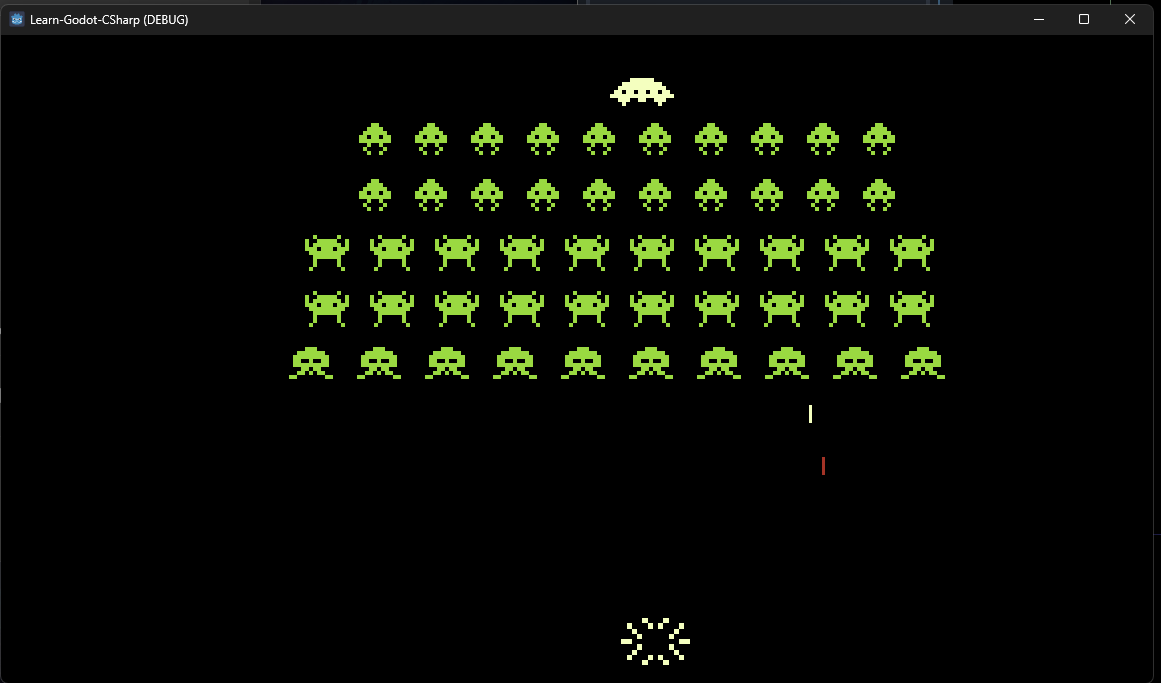
\includegraphics[width=1\textwidth]{ImplementatieSpel.png}
    \caption{Implementatie}
    \label{fig:POC}
\end{figure}


%\input{...}
%...

%%=============================================================================
%% Conclusie
%%=============================================================================

\chapter{Conclusie}%
\label{ch:conclusie}

% TODO: Trek een duidelijke conclusie, in de vorm van een antwoord op de
% onderzoeksvra(a)g(en). Wat was jouw bijdrage aan het onderzoeksdomein en
% hoe biedt dit meerwaarde aan het vakgebied/doelgroep? 
% Reflecteer kritisch over het resultaat. In Engelse teksten wordt deze sectie
% ``Discussion'' genoemd. Had je deze uitkomst verwacht? Zijn er zaken die nog
% niet duidelijk zijn?
% Heeft het onderzoek geleid tot nieuwe vragen die uitnodigen tot verder 
%onderzoek?
Om de onderzoeksvraag te beantwoorden: "Welke 2D game-engines zijn geschikt voor programmeurs van AllPhi met een C\# achtergrond, maar zonder game development-ervaring, om games te ontwikkelen voor evenementen?", biedt de ontwikkeling van de proof-of-concept waardevolle inzichten. Godot blijkt een toegankelijke instap voor het leren ontwikkelen van games, waarbij de ondersteuning voor C\# voldoende is gebleken voor het creëren van eenvoudige videogames.

%---------- Bijlagen -----------------------------------------------------------

\appendix

\chapter{Onderzoeksvoorstel}

Het onderwerp van deze bachelorproef is gebaseerd op een onderzoeksvoorstel dat vooraf werd beoordeeld door de promotor. Dat voorstel is opgenomen in deze bijlage.

%% TODO: 
%\section*{Samenvatting}

% Kopieer en plak hier de samenvatting (abstract) van je onderzoeksvoorstel.

% Verwijzing naar het bestand met de inhoud van het onderzoeksvoorstel
%---------- Inleiding ---------------------------------------------------------

\section{Introductie}%
\label{sec:introductie}

AllPhi is een technologiebedrijf dat elk jaar aanwezig is op een aantal technologiebeurzen. Op deze beurzen organiseert AllPhi een interactieve challenge voor bezoekers. De winnaar van de challenge ontvangt een leuke prijs.

Voor de meest recente editie van de challenge ontwikkelde AllPhi een eigen Snake-spel. Dit spel was ontwikkeld met behulp van C\# en .NET. Hoewel AllPhi geen professionele gameontwikkelaars zijn, waren ze tevreden met het resultaat.

Om in de toekomst nog betere challenges te kunnen ontwikkelen, wil AllPhi onderzoeken welke game engine het makkelijkst te gebruiken is voor mensen met een achtergrond in C\# en .NET, maar geen game development achtergrond hebben.


%---------- Stand van zaken ---------------------------------------------------

\section{State-of-the-art}%
\label{sec:state-of-the-art}
\subsection{Game engines}
Game engines zijn een cruciaal element in de game development wereld. Deze vergemakkelijken het ontwikkelen van videospellen. Ze bieden varierende tools aan om dit te bereiken. Van animaties tot gebruikers interacties tot detectie van botsingen. Volgens \textcite{Barczak2021} is een game engine een software toolkit die productie van games op verschillende platformen vereenvoudigt.

\subsection{Unity}
Unity is een commerciële game engine die een breed scala aan features biedt, waaronder ondersteuning voor 2D- en 3D-graphics, fysica, geluid, netwerken en augmented reality.\autocite{Haas2014} Unity is echter ook duurder en heeft een hogere leercurve dan Godot.

\subsection{Godot}
Godot onderscheidt zich als een volledig uitgeruste, moderne game engine die een unieke combinatie van toegankelijkheid en flexibiliteit biedt. Als een gratis en open-source platform, biedt Godot een hoger niveau van transparantie in vergelijking met commerciële alternatieven zoals Unity. Deze openheid zorgt ervoor dat er geen functionaliteiten verborgen zijn achter een betaalmuur, wat een belangrijk voordeel is voor ontwikkelaars die met budgetbeperkingen werken.\autocite{Bradfield2018}

Godot's open-source karakter zorgt ook voor een actieve en ondersteunende gemeenschap. Deze gemeenschap speelt een cruciale rol bij het voortdurend verbeteren van de engine, het bijdragen aan documentatie, en het delen van kennis, wat van onschatbare waarde is voor zowel nieuwe als ervaren gebruikers.

% Voor literatuurverwijzingen zijn er twee belangrijke commando's:
% \autocite{KEY} => (Auteur, jaartal) Gebruik dit als de naam van de auteur
%   geen onderdeel is van de zin.
% \textcite{KEY} => Auteur (jaartal)  Gebruik dit als de auteursnaam wel een
%   functie heeft in de zin (bv. ``Uit onderzoek door Doll & Hill (1954) bleek
%   ...'')

%---------- Methodologie ------------------------------------------------------
\section{Methodologie}
\label{sec:methodologie}

Deze studie gebruikt een vergelijkende benadering om twee identieke 2D-platformspellen te ontwikkelen, elk met behulp van een andere game engine: Godot en Unity. Het primaire doel is het onderzoeken van een scala aan variabelen, waaronder gebruiksgemak, leercurve voor beginners, technologische integratie, tijd benodigd voor implementatie, en de totale gebruikerservaring. Hieronder volgt een gedetailleerd overzicht van de geplande functionaliteiten van de spellen en de evaluatiecriteria.

In de eerste fase worden beide game engines geïnstalleerd, waarvoor een periode van één week is gereserveerd. Voor de implementatie van elke functionaliteit wordt vervolgens 1 tot 2 weken uitgetrokken. Dit tijdsbestek zorgt ervoor dat er voldoende ruimte is om elke functie in beide engines te implementeren en de resultaten grondig te analyseren.

\subsection{Functionaliteiten voor de Proof-of-Concept Spellen}

De proof-of-concept spellen zullen worden voorzien van diverse essentiële kenmerken om een representatieve vergelijking tussen Godot en Unity mogelijk te maken. Deze kenmerken omvatten:

\begin{itemize}
    \item \textbf{Beweging:} Het karakter kan bewegen naar links en rechts met behulp van de pijltoetsen of WASD-toetsen.
    \item \textbf{Wereld:} Het eerste level vindt plaats in een 2D-wereld met blokken en andere objecten.
    \item \textbf{Springen en Duiken:} Het karakter kan acties uitvoeren zoals springen en duiken.
    \item \textbf{Interactie met Blokken:} Het karakter kan interageren met omgevingsblokken, bijvoorbeeld klimmen, verplaatsen of vernietigen.
    \item \textbf{Interactie met Vijanden:} Het karakter kan vijanden verslaan of ontwijken.
    \item \textbf{Scoresysteem:} Een systeem dat scores berekent op basis van verslagen vijanden en verzamelde blokken.
    \item \textbf{Levelselectie:} Een menu om verschillende speellevels te selecteren.
    \item \textbf{Moeilijkheidsgraden:} Verschillende moeilijkheidsniveaus aangepast aan de vaardigheden van de speler.
\end{itemize}

Elke functionaliteit wordt afwisselend eerst in één van de twee engines geïmplementeerd. Na implementatie in beide engines worden de volgende criteria geëvalueerd:
\begin{itemize}
    \item \textbf{Implementatietijd:} De tijd benodigd voor de implementatie van elke functionaliteit.
    \item \textbf{Leerdurve:} De moeilijkheidsgraad bij het implementeren van de functionaliteit.
    \item \textbf{Gebruikerstests:} Deze worden uitgevoerd om de gebruikerservaring van beide game engines te evalueren.
\end{itemize}

Deze methodologische aanpak biedt een gestructureerde en evenwichtige vergelijking van de twee game engines, wat waardevolle inzichten zal leveren voor toekomstige projecten in gameontwikkeling.


%---------- Verwachte resultaten ----------------------------------------------
\section{Verwacht resultaat, conclusie}%
\label{sec:verwachte_resultaten}

De gebruikersinterface van Godot onderscheidt zich door haar eenvoud en intuïtieve design, wat in het bijzonder gunstig lijkt voor beginnende ontwikkelaars die zich richten op 2D-platformers. Godot's specialisatie in dit genre belooft een soepelere leercurve. Aan de andere kant staat Unity bekend om zijn robuustheid en uitgebreide bronnen, dankzij een langere aanwezigheid in de industrie. Deze factoren maken Unity een aantrekkelijke optie voor complexere projecten. Echter, voor aspirant-ontwikkelaars zonder eerdere ervaring in game-ontwikkeling lijkt Godot de meer toegankelijke keuze te zijn.




%%---------- Andere bijlagen --------------------------------------------------
% TODO: Voeg hier eventuele andere bijlagen toe. Bv. als je deze BP voor de
% tweede keer indient, een overzicht van de verbeteringen t.o.v. het origineel.
%\input{...}

%%---------- Backmatter, referentielijst ---------------------------------------

\backmatter{}

\setlength\bibitemsep{2pt} %% Add Some space between the bibliograpy entries
\printbibliography[heading=bibintoc]

\end{document}
